\section{Dataset}
\label{chap:dataset}

L’accurata definizione e preparazione dei dataset rappresenta una fase cruciale in ogni studio sperimentale basato su tecniche di \textbf{machine learning}, ancor più quando si opera in ambiti ad alta sensibilità come la \textbf{Digital Forensics}. In questo contesto, l’obiettivo della sperimentazione è valutare la \textbf{robustezza operativa} di strumenti di classificazione automatica di immagini contenenti armi, esposti a perturbazioni intenzionali a fini \textit{adversariali} o anti-forensi.

Per supportare tale analisi, è stata sviluppata una collezione di \textbf{cinque dataset} tematicamente coerenti ma eterogenei per origine, struttura e livello di realismo. Alcuni sono stati selezionati da fonti pubbliche esistenti (Kaggle, repository open-source), altri costruiti ex-novo tramite \textbf{scraping automatizzato} da web surface, social network e deep web. Questa diversificazione è funzionale a valutare l’efficacia degli algoritmi in scenari sia controllati sia non supervisionati, riflettendo le complessità operative di casi reali.

Ciascun dataset è stato organizzato secondo il paradigma di \textbf{classificazione supervisionata}, ove possibile, e sottoposto a operazioni di pulizia e verifica dell’integrità. Le immagini raccolte includono contesti realistici, simulati e non strutturati, offrendo una \textbf{variabilità visiva significativa} per testare le capacità di generalizzazione e resilienza dei modelli AI.

Nel presente capitolo vengono descritti in dettaglio i cinque dataset selezionati e costruiti, riportando per ciascuno le modalità di acquisizione, la struttura delle classi, il numero di immagini e il codice utilizzato per l’estrazione automatica, ove applicabile.











\subsection*{Descrizione della composizione del Dataset}
\label{sec:descrizione-dataset}

La presente tesi sperimentale si fonda sull’analisi della \textbf{robustezza operativa} di strumenti basati su Intelligenza Artificiale per la classificazione automatica di immagini in ambito forense, esposti a input manipolati tramite tecniche \textit{anti-forensi} e \textit{adversariali}. Per valutare tale robustezza in uno scenario realistico, è stato costruito un dataset composito di \textbf{1000 immagini} etichettate manualmente come contenenti o meno armi, integrando dati provenienti da fonti eterogenee e rappresentative di diversi contesti operativi.

In particolare, sono stati selezionati e normalizzati cinque sotto-dataset, ciascuno caratterizzato da una diversa modalità di raccolta, struttura semantica e livello di qualità visiva:

\begin{itemize}
\item \textbf{Dataset 1 – Weapon Detection Dataset (Kaggle):} raccolta strutturata con 9 classi di armi, utile come base per la classificazione supervisionata.
\item \textbf{Dataset 2 – DeepFirearm Subset:} estratto controllato da dataset open-source, focalizzato su modelli specifici di armi da fuoco.
\item \textbf{Dataset 3 – Raccolta personalizzata tramite scraping:} immagini provenienti da Google Images per classi tematiche simulate ad alto rumore.
\item \textbf{Dataset 4 – OSINT da YouTube e fonti aperte:} immagini reali estratte da thumbnail video o fonti non strutturate.
\item \textbf{Dataset 5 – Deep Web:} raccolta mirata da archivi .onion tramite scraping, orientata a testare i modelli su contenuti \textit{non convenzionali}.
\end{itemize}

L’obiettivo di tale composizione è duplice: da un lato ottenere una \textbf{base eterogenea e bilanciata} su cui testare la resilienza dei modelli di classificazione in condizioni realistiche; dall’altro esplorare \textbf{l’impatto delle sorgenti non tradizionali} (deep web, OSINT, scraping) sulle prestazioni e sulla vulnerabilità degli strumenti AI-based. Ogni dataset è stato sottoposto a verifica di integrità, ristrutturazione e annotazione manuale per garantire coerenza semantica nell’etichettatura binaria (arma / non arma), indipendentemente dalla fonte originaria.


\subsection*{Considerazioni quantitative sui test avversariali}
Il corpus complessivo utilizzato in questa tesi comprende oltre \textbf{5000 immagini}, raccolte da fonti eterogenee e suddivise in cinque dataset. Tuttavia, per motivi computazionali, le tecniche di perturbazione avversariale verranno applicate solo a un sottoinsieme selezionato.

\begin{itemize}
    \item Verranno selezionate circa \textbf{1000 immagini pulite totali}, equamente distribuite tra dataset strutturati (es. Kaggle, DeepFirearm) e non strutturati (es. Telegram, deep web).
    \item Ogni strumento AI-based  testato sarà sottoposto alla verifica su circa \textbf{10000 immagini perturbate}, suddivise tra le principali tecniche adottate (\texttt{FGSM}, \texttt{SuperDeepFool}, \texttt{Color Shifting}, ecc.).
    \item Verranno incluse immagini \textbf{fuori distribuzione} (OOD), rumorose o ambigue, per misurare l’effettiva resilienza del sistema in contesti operativi complessi.
\end{itemize}

Questo approccio è coerente con quanto suggerito nella letteratura scientifica~\cite{goodfellow2014explaining,biggio2018wild}, secondo cui l’uso di subset bilanciati e realistici è sufficiente a produrre valutazioni attendibili sull'efficacia e la robustezza dei modelli AI esposti ad attacchi.



\subsection*{Dataset 1: Weapon Detection Dataset (Kaggle)}
Il primo dataset considerato per l’analisi sperimentale è il \textbf{Weapon Detection Dataset} \cite{Sanyal2023KaggleWeapon}, reso disponibile tramite la piattaforma \textbf{Kaggle}.\footnote{\url{https://www.kaggle.com/}} Questo dataset è stato concepito per supportare la classificazione automatica di immagini contenenti armi, in contesti visivi realistici.

Il dataset comprende circa \textbf{1000 immagini}, suddivise in \textbf{9 categorie distinte}: \texttt{Handgun}, \texttt{Rifle}, \texttt{Shotgun}, \texttt{SMG}, \texttt{Knife}, \texttt{Sword}, \texttt{Sniper}, \texttt{Bazooka}, \texttt{Grenade Launcher}. Le immagini sono organizzate in cartelle separate per ciascuna classe e sono in formato JPEG, con una buona variabilità in termini di background, orientamento e qualità visiva.

Questa collezione è particolarmente utile non solo per addestrare modelli di deep learning alla classificazione di armi da fuoco, ma anche per la valutazione della loro \textbf{robustezza operativa} in presenza di immagini modificate tramite tecniche di \textbf{adversarial perturbation}.





\subsection*{Dataset 2: Sottocampionamento da DeepFirearm}
Il secondo dataset è stato ricavato tramite un \textbf{sottocampionamento controllato} del dataset open-source \texttt{DeepFirearm} \cite{Hao2018DeepFirearm}, una collezione di immagini di armi da fuoco suddivise per modello. Il dataset originale contiene oltre 100 classi, ma presenta un'elevata eterogeneità sia in termini di contenuto visivo sia di distribuzione numerica.

Per la selezione è stato applicato un criterio automatico: sono state incluse solo le classi con almeno 20 immagini disponibili, limitando il numero massimo a \textbf{200 immagini per classe}, fino a un massimo di circa \textbf{1000 immagini}. L’output finale comprende \textbf{13 classi} e \textbf{1013 immagini}.

Le classi selezionate includono varietà storiche e moderne, tra cui: \texttt{1853 Enfield rifle-musket}, \texttt{AEK-919K}, \texttt{AK-47}, \texttt{AK-12}, \texttt{AN-94}, \texttt{AS Val}, \texttt{Astra 600}, \texttt{Berdan Sharps Rifle}, \texttt{Beretta M9A1}, \texttt{Brown Bess musket}, \texttt{Browning BT-99 Shotgun}, \texttt{Browning Hi-Power Mark III} e \texttt{COLT WOODSMAN}.

Tutte le immagini sono state organizzate in sottodirectory per ciascuna classe, secondo un paradigma di classificazione \textbf{supervisionata}. Questo dataset permette di testare modelli AI in scenari realistici e bilanciati, mantenendo una buona rappresentatività di armi di diverso tipo e provenienza.
Il codice Python utilizzato per la selezione automatica delle classi dal dataset \texttt{DeepFirearm} è riportato in \textbf{Appendice~\ref{appendice:code}}, \texttt{Codice~\ref{lst:python_DB2}}.





\subsection*{Dataset 3: Raccolta personalizzata tramite scraping}
Il terzo dataset è stato costruito mediante un processo di \textbf{web scraping controllato} da \texttt{Google Images}, utilizzando la libreria \texttt{icrawler}. Sono state definite quindici classi tematiche simulate, tra cui \texttt{concealed weapon}, \texttt{gun on table}, \texttt{toy gun}, \texttt{airsoft weapon}, \texttt{damaged firearm}, e altre. Ogni classe rappresenta uno scenario potenzialmente ambiguo, realistico o operativo, particolarmente rilevante in ambito forense.

Sono state raccolte automaticamente almeno \textasciitilde1000 immagini, distribuite tra le classi selezionate, ciascuna delle quali è stata salvata in una directory separata secondo un paradigma di classificazione \textbf{supervisionata}. Al termine della raccolta, le immagini sono state sottoposte a un processo di \textbf{validazione di integrità} per rimuovere file corrotti o non interpretabili.

Questa raccolta, per sua natura \textbf{non strutturata} e derivante da fonti pubblicamente accessibili, introduce un’elevata \textbf{eterogeneità visiva}, cruciale per simulare \textbf{condizioni operative complesse e non controllate} nella classificazione automatizzata in contesto forense.

Per la raccolta automatica tramite scraping da \texttt{Google Images} è stato sviluppato uno script Python, consultabile in \textbf{Appendice~\ref{appendice:code}}, \texttt{Codice~\ref{lst:python_DB3}}.





\subsection*{Dataset 4: Raccolta OSINT da YouTube e fonti aperte}
Questo dataset è stato costruito mediante una strategia \textbf{OSINT} (Open Source Intelligence), basata sull’acquisizione di thumbnail da video YouTube pubblicamente accessibili. In caso di errore o indisponibilità del contenuto, è stato attivato un meccanismo automatico di \textbf{fallback} tramite \texttt{Google Images}, usando ricerche semantiche equivalenti.

Le immagini, sebbene meno strutturate rispetto a dataset annotati, rappresentano un’importante fonte di \textbf{informazione realistica} e \textbf{non supervisionata}, utile per la valutazione della \textbf{capacità di generalizzazione} e della \textbf{robustezza} dei modelli AI in scenari complessi e dinamici.

La pipeline OSINT basata su \texttt{Telegram} e \texttt{YouTube} è descritta nel codice Python riportato in \textbf{Appendice~\ref{appendice:code}}, \texttt{Codice~\ref{lst:python_DB4}}.





\subsection*{Dataset 5: Raccolta dal Deep Web}
Il quinto dataset è stato costruito tramite accesso a contenuti open source presenti su piattaforme non indicizzate (deep web), principalmente forum, mercati e archivi .onion. La raccolta è stata condotta nel rispetto dei principi etici della ricerca scientifica e delle normative vigenti, evitando ogni contenuto illegale o lesivo.

Le immagini sono state etichettate manualmente secondo contesti d’uso specifici, come \texttt{weapon showcase}, \texttt{concealed carry}, \texttt{modifiche artigianali}, \texttt{armi in ambienti domestici}. Questa raccolta consente di testare i modelli AI su \textbf{contenuti non convenzionali}, frequentemente assenti nei dataset pubblici.

La raccolta da fonti \texttt{deep web} è stata effettuata tramite uno script custom, riportato in \textbf{Appendice~\ref{appendice:code}}, \texttt{Codice~\ref{lst:python_DB5}}.






\subsection*{Immagini selezionate per la valutazione di robustezza: Clean Dataset}
\label{subsec:dataset_finale}

Per la valutazione sperimentale della robustezza operativa dei classificatori AI-based in ambito forense, è stato costruito un dataset bilanciato e rappresentativo a partire da cinque sorgenti eterogenee. Ogni sorgente è stata scelta per riflettere una specifica modalità di acquisizione realistica: da dataset pubblici pre-strutturati a immagini estratte da social network e ambienti deep web, simulando così la varietà tipica dei contesti investigativi.

Sono state selezionate manualmente \textbf{200 immagini per ciascun dataset}, per un totale complessivo di \textbf{1000 immagini}. Ogni immagine è stata verificata per garantire:
\begin{itemize}
    \item l'integrità del file e la corretta leggibilità da parte degli strumenti di analisi automatica;
    \item dimensioni visive comprese in intervalli adeguati per l'elaborazione (nessuna immagine è risultata corrotta o eccessivamente piccola);
    \item un equilibrio semantico e una varietà tematica (tipologia d'arma, contesto visivo, angolazione).
\end{itemize}

\begin{table}[H]
\centering
\caption{Statistiche riassuntive delle immagini selezionate per ciascun dataset. Ogni dataset include esattamente 200 immagini, verificate manualmente per qualità e leggibilità. Le dimensioni medie e totali sono espresse rispettivamente in pixel e megabyte (MB).}
\label{tab:dataset_stats}
\begin{tabularx}{\textwidth}{l>{\raggedleft\arraybackslash}X>{\raggedleft\arraybackslash}X>{\raggedleft\arraybackslash}X>{\raggedleft\arraybackslash}X>{\raggedleft\arraybackslash}X}
\toprule
\textbf{Dataset} & \textbf{Larghezza media [px]} & \textbf{Altezza media [px]} & \textbf{Dim. media [kB]} & \textbf{Dim. totale [MB]} & \textbf{Immagini} \\
\midrule
01\_archive (Kaggle) & 1372.63 & 1012.87 & 327.75 & 62.5 & 200 \\
02\_github\_deep\_firearm & 1184.66 & 755.62 & 326.64 & 62.3 & 200 \\
03\_scraped\_firearm\_dataset & 1375.39 & 1132.40 & 500.10 & 95.4 & 200 \\
04\_Osint\_yt\_telegram & 1046.93 & 887.52 & 179.21 & 34.2 & 200 \\
05\_deepweb\_dataset & 585.32 & 482.82 & 140.20 & 26.7 & 200 \\
\bottomrule
\end{tabularx}
\end{table}

La Tabella~\ref{tab:dataset_stats} riassume le statistiche fondamentali del dataset finale, riportando per ciascuna sorgente la dimensione media delle immagini (in pixel), la dimensione media del file in kilobyte e il peso totale in megabyte.

Tale collezione costituisce il \textbf{test set ufficiale} utilizzato per le valutazioni comparative di robustezza. Il suo impiego ha consentito di testare i classificatori AI in condizioni realistiche ma controllate, permettendo l'applicazione sistematica di perturbazioni adversariali e manipolazioni anti-forensi.



Tutti i file sono stati raccolti e organizzati nella directory \texttt{Test\_Dataset}, suddivisa in sottocartelle corrispondenti alle cinque fonti originarie:
\begin{enumerate}
    \item \texttt{01\_archive} – Weapon Detection Dataset da Kaggle;
    \item \texttt{02\_github\_deep\_firearm} – Sottoselezione dal dataset DeepFirearm;
    \item \texttt{03\_scraped\_firearm\_dataset} – Dataset costruito tramite scraping da motori di ricerca;
    \item \texttt{04\_osint\_yt\_telegram} – Raccolta da gruppi Telegram e video pubblicati su YouTube;
    \item \texttt{05\_deepweb\_dataset} – Raccolta automatica da siti del deep web tramite rete Tor.
\end{enumerate}

Questa struttura bilanciata consente di valutare la tenuta dei sistemi di classificazione su immagini provenienti da contesti molto diversi tra loro, garantendo una validazione esterna più solida e realistica rispetto a benchmark sintetici o omogenei. L'estrazione automatizzata dai dataset descritti nelle sezioni precedenti è stata effettuata mediante uno script personalizzato, che ha permesso di filtrare, selezionare e strutturare le immagini in modo coerente con i vincoli sperimentali.
Tale codice è riportato in \textbf{Appendice~\ref{appendice:code}}, \texttt{Codice~\ref{lst:python_DBSubSetChoice}}.







\subsection*{Validazione e pre-processing delle immagini selezionate}
I dataset derivanti da \textbf{scraping automatico} — in particolare quelli raccolti tramite \texttt{Google Images} e da fonti nel \texttt{deep web} — sono stati sottoposti a una fase preliminare di \textbf{validazione} e \textbf{filtro di qualità}, finalizzata a garantire l'affidabilità e la coerenza delle immagini incluse nel corpus.

In questa fase, sono stati implementati i seguenti controlli automatici:

\begin{itemize}
    \item \textbf{Verifica dell'integrità}: esclusione di immagini corrotte o non leggibili, tramite apertura e validazione con la libreria \texttt{PIL}.
    \item \textbf{Rimozione di duplicati}: confronto basato su hash \texttt{MD5} del contenuto binario, al fine di identificare copie esatte.
    \item \textbf{Controllo della risoluzione}: scarto di immagini con dimensione inferiore a \texttt{300px} in larghezza o altezza.
    \item \textbf{Esclusione di contenuti non pertinenti}: filtraggio euristico di file contenenti elementi ricorrenti come loghi, banner, captcha o icone, sulla base di pattern nei nomi dei file o nel percorso di origine.
\end{itemize}

Tali procedure non sono state applicate ai dataset già strutturati e annotati (es. Kaggle e DeepFirearm), poiché già validati a monte. La validazione automatica dei dataset raccolti tramite scraping ha contribuito in modo determinante alla creazione di un insieme di immagini di alta qualità, essenziale per condurre esperimenti di classificazione e test di robustezza in scenari realistici.






\subsection*{Criterio di selezione dimensionale}
\label{sec:criterio-dimensione}

Durante la fase di costruzione del dataset è stata adottata una soglia minima sulle dimensioni delle immagini pari a \textbf{300X300 pixel}. Questa scelta metodologica è stata motivata da considerazioni sia tecniche che empiriche, legate alla compatibilità con i modelli di deep learning utilizzati e alla qualità semantica delle informazioni visive contenute nelle immagini.

In particolare, la maggior parte dei modelli di classificazione pre-addestrati, come ResNet o Vision Transformer (ViT), richiedono come input immagini di dimensione minima pari a \textbf{224X224 pixel}. Tale requisito deriva dal fatto che le architetture sono state addestrate su dataset benchmark (es. ImageNet) normalizzati a tale risoluzione:

\begin{quote}
\textit{"All input images are resized to 224X224 using bicubic interpolation before being passed to the ResNet models."} \\ 
\small -- He et al., Deep Residual Learning for Image Recognition, CVPR 2016\cite{he2016deep}.
\end{quote}

Nel caso specifico del modello \textbf{CLIP ViT-B/32} impiegato per la classificazione automatica, la risoluzione standard di riferimento è pari a \textbf{224X224 pixel}, rendendo necessario un dimensionamento minimo compatibile:

\begin{quote}
\textit{"We use the ViT-B/32 variant with an input resolution of 224X224."} \\ 
\small -- Radford et al., Learning Transferable Visual Models From Natural Language Supervision, ICML 2021~\cite{radford2021learning}.
\end{quote}

Oltre ai requisiti architetturali, diverse evidenze sperimentali in letteratura confermano che una bassa risoluzione influisce negativamente sull’accuratezza dei modelli, in particolare nei compiti di classificazione fine-grained:

\begin{quote}
\textit{"Low-resolution inputs lead to notable degradation in classification accuracy, particularly in fine-grained tasks."} \\ 
\small -- Tan et al., EfficientNet: Rethinking Model Scaling for Convolutional Neural Networks, ICML 2019~\cite{tan2019efficientnet}.
\end{quote}

Pertanto, la soglia di \textbf{300 pixel} è stata scelta come compromesso ragionato per:

\begin{itemize}
  \item garantire compatibilità piena con i modelli pre-addestrati basati su ImageNet o simili;
  \item ridurre la perdita informativa dovuta a upscaling e interpolazioni eccessive;
  \item preservare un livello minimo di qualità semantica e visiva dell'immagine.
\end{itemize}

Questa strategia ha permesso di filtrare automaticamente immagini troppo piccole, sfocate o frammentarie, migliorando così la qualità complessiva del dataset e la robustezza del processo di addestramento e valutazione sperimentale.






\subsection*{Rilevanza delle immagini non rilevanti nei test adversariali}
Nel contesto della presente ricerca, la decisione di mantenere immagini non strettamente pertinenti nel corpus sperimentale non rappresenta una debolezza metodologica, bensì una scelta intenzionale e strategica.

In scenari reali, i sistemi di classificazione automatica sono frequentemente esposti a \textbf{input fuori distribuzione} (OOD) o \textbf{rumore semantico e visivo}, ovvero immagini che non appartengono alle classi addestrate ma che possono attivare risposte errate nei modelli. Questo comportamento, se combinato con perturbazioni \textit{adversariali}, può amplificare drasticamente la vulnerabilità del sistema, favorendo attacchi mirati su immagini già ambigue o borderline.

Diversi studi~\cite{hendrycks2017baseline,fort2021exploring} sottolineano l'importanza di includere campioni OOD durante la valutazione dei modelli, al fine di stimare la reale robustezza del sistema in contesti operativi non controllati.

Nel caso di dataset costruiti tramite scraping (deep web, Telegram, web search), tale variabilità è strutturalmente presente e viene considerata parte integrante della pipeline di validazione sperimentale. L’inclusione di immagini non rilevanti permette quindi di:

\begin{itemize}
    \item simulare scenari \textbf{open-world}, tipici della digital forensics e dell’OSINT investigativo;
    \item stressare i modelli durante i test \textbf{adversariali} su input non canonici;
    \item osservare fenomeni di \textbf{overconfidence} o errore sistematico in presenza di ambiguità visiva.
\end{itemize}


\vspace{0.5cm}








\subsection*{Gestione delle immagini non rilevanti}
Durante il processo di raccolta automatica di immagini da fonti aperte e non strutturate (come scraping web e deep web), è stato inevitabile includere una quota di immagini non rilevanti rispetto al dominio specifico di interesse, ovvero la rappresentazione visiva di armi da fuoco e strumenti simili.

Tali immagini possono raffigurare oggetti comuni, elementi decorativi, simboli, fotografie personali o immagini di bassa qualità che non contengono armi. La decisione se rimuoverle o mantenerle è stata oggetto di riflessione metodologica.

\textbf{Nel contesto di questa tesi, è stato scelto di \underline{non rimuovere a priori} tutte le immagini non pertinenti.} Questa scelta si fonda su diverse considerazioni tecniche:

\begin{itemize}
\item \textbf{Realismo operativo:} in uno scenario reale di applicazione, i modelli di classificazione automatica sono frequentemente esposti a immagini fuori dominio, ambigue o ambivalenti. La presenza di immagini non rilevanti nel dataset addestrativo o di test può simulare condizioni realistiche di rumore semantico e visuale, contribuendo a valutare la \textbf{robustezza del sistema} e la sua capacità di generalizzazione.

\item \textbf{Non-supervised filtering costoso:} la rimozione automatica di immagini non rilevanti richiederebbe l’impiego di classificatori già addestrati o reti neurali pre-esistenti, introducendo una forma di \textit{bias} che risulterebbe in contrasto con l'obiettivo di valutare le performance in condizioni neutre e non assistite.

\item \textbf{Valore nei falsi positivi:} alcune immagini, pur non rappresentando armi, possono essere erroneamente classificate come tali. Questi casi sono preziosi per analizzare la sensibilità del modello agli \textbf{errori di classificazione} e la sua suscettibilità a input ambigui, in particolare in presenza di attacchi adversariali.

\item \textbf{Sostenibilità computazionale:} operare una selezione manuale o semi-automatica su migliaia di immagini avrebbe comportato un overhead temporale non giustificato rispetto al guadagno informativo ottenuto, dato che la presenza di rumore è stata considerata parte integrante della valutazione sperimentale.
\end{itemize}

Nel caso specifico del dataset raccolto dal deep web, l’eterogeneità dei contenuti e la mancanza di annotazioni formali sono caratteristiche intrinseche che riflettono le condizioni operative di un ambiente non strutturato. Includere immagini spurie permette di \textbf{testare l'efficacia dei modelli in condizioni non ideali}, e di osservare come si comportano rispetto a contenuti \textit{out-of-distribution} (OOD).





\subsection{Strumenti AI per la classificazione automatica: CLIP, BLIP, EfficientNet e ResNet+SVM}
\label{sec:modelli-ai-classificazione}

L’impiego di strumenti basati su \textbf{Intelligenza Artificiale (AI)} per la \textit{classificazione automatica di immagini} costituisce uno degli ambiti più rilevanti e maturi dell’odierna ricerca nel campo del Deep Learning. Questi strumenti permettono di assegnare in modo automatico un’etichetta semantica a un contenuto visivo sulla base delle regolarità apprese da grandi dataset durante la fase di addestramento. In contesto forense, la classificazione automatica si presta a numerose applicazioni operative, tra cui il riconoscimento di oggetti sospetti, armi, volti o scene di rilevanza investigativa ~\cite{nowroozi2020adversarial, costantini2019digital}.

Dal punto di vista tecnico, un classificatore automatico per immagini è composto da due elementi fondamentali: una \textbf{funzione di rappresentazione}, ovvero un modello che estrae embedding semantici dalle immagini (di solito una rete neurale convoluzionale o un transformer visivo), e una \textbf{funzione di decisione}, che assegna un’etichetta discreta alla rappresentazione prodotta. I sistemi moderni combinano spesso queste due componenti in architetture end-to-end, in grado di apprendere sia le feature che la decisione finale durante il processo di training ~\cite{bishop2006pattern}.

Recentemente, l’integrazione di modelli \textit{multimodali} ha ulteriormente esteso la capacità di questi strumenti, consentendo di associare contenuti visivi a descrizioni testuali in linguaggio naturale e di operare anche in scenari zero-shot, in cui le classi di output non sono presenti nei dati di addestramento. In tale prospettiva, modelli come \textbf{CLIP} e \textbf{BLIP} hanno dimostrato notevole efficacia, ponendosi come alternative flessibili e semanticamente robuste rispetto ai classificatori tradizionali.

Nel presente lavoro sono stati selezionati quattro strumenti AI per la classificazione binaria (arma / non arma), rappresentativi di diverse famiglie architetturali:

\paragraph{CLIP ViT-B/32 (OpenAI).} CLIP (Contrastive Language–Image Pre-training) è un modello multimodale sviluppato da OpenAI \cite{radford2021learning}, addestrato su un ampio corpus di immagini e descrizioni testuali mediante apprendimento contrastivo. La variante ViT-B/32 utilizza un Transformer visivo di tipo Vision Transformer (ViT) \cite{dosovitskiy2020image} con patch di dimensione 32, ed è in grado di mappare immagini e testi in uno spazio semantico condiviso.  
\textit{In questa tesi, CLIP è stato scelto per valutare la robustezza di classificatori zero-shot in scenari realistici e non supervisionati, dove le immagini possono essere fuori distribuzione o ambigue. Il modello è inoltre stato impiegato come strumento preliminare per supportare l’annotazione manuale delle immagini.}

\paragraph{BLIP (Bootstrapped Language-Image Pretraining).} BLIP è un framework multimodale proposto da Salesforce AI Research \cite{li2020learning}, che integra il pretraining contrastivo con un approccio captioning-aware, finalizzato a generare descrizioni testuali coerenti e classificazioni semantiche.  
\textit{Il suo impiego nella tesi è finalizzato a verificare quanto modelli di captioning possano mantenere accuratezza semantica in presenza di perturbazioni visive, e se le descrizioni generate siano vulnerabili a tecniche anti-forensi o adversariali.}

\paragraph{EfficientNet-B0.} EfficientNet è una famiglia di reti convoluzionali introdotta da Google AI \cite{tan2019efficientnet}, nota per l’equilibrio ottimale tra accuratezza e costo computazionale. La versione B0 rappresenta la configurazione base, derivata tramite Neural Architecture Search (NAS).  
\textit{In questo lavoro, EfficientNet-B0 è stato fine-tuned come modello supervisionato, fornendo una baseline moderna e compatta per valutare l’impatto delle perturbazioni visive standard (es. occlusione, sfocatura, compressione JPEG).}

\paragraph{ResNet18 + SVM.} Come baseline classica è stato implementato un classificatore a due fasi: estrazione delle feature visive tramite ResNet18 ~\cite{he2016deep}, seguita dall’addestramento di un classificatore lineare SVM (Support Vector Machine) \cite{cortes1995support}.  
\textit{Questa configurazione è stata adottata per offrire un confronto diretto con modelli più recenti. Il suo approccio modulare e interpretabile permette di osservare l’impatto separato delle perturbazioni sulla fase di rappresentazione (feature extraction) e sulla decisione finale.}

\bigskip

La scelta di modelli appartenenti a paradigmi architetturali eterogenei permette una comparazione critica più ampia in termini di accuratezza, robustezza e sensibilità agli attacchi adversariali o anti-forensi. Tale confronto si pone come obiettivo centrale per comprendere l’affidabilità e la sicurezza operativa degli strumenti AI impiegati in scenari forensi reali, dove la presenza di immagini manipolate o non conformi alla distribuzione attesa può compromettere seriamente la validità del processo decisionale automatizzato.



\begin{table}[H]
  \centering
  \caption{Confronto tra i modelli AI utilizzati per la classificazione automatica (arma / non arma).}
  \label{tab:modelli-ai-confronto}
  \begin{tabularx}{\textwidth}{>{\raggedright\arraybackslash}p{3cm} >{\raggedright\arraybackslash}p{2.5cm} >{\raggedright\arraybackslash}p{2.5cm} >{\raggedright\arraybackslash}p{2.5cm} >{\raggedright\arraybackslash}X}
  \toprule
  \textbf{Modello} & \textbf{Tipo / Architettura} & \textbf{Input} & \textbf{Output} & \textbf{Output atteso} \\
  \midrule
  \textbf{CLIP ViT-B/32} & Multimodale \\ (ViT Transformer + Text Encoder) & Immagine + prompt testuale & Classe più compatibile tra le label testuali predefinite & Etichetta binaria assegnata in modalità zero-shot in base alla similarità semantica immagine-testo (es. ``arma'' o ``non arma'') \\
  \addlinespace
  \textbf{BLIP} & Multimodale encoder-decoder \\ (Vision Transformer + GPT-like LM) & Immagine & Caption descrittiva + analisi testuale & Didascalia generata automaticamente da cui si deduce la presenza o meno di un’arma reale tramite keyword filtering o parsing semantico \\
  \addlinespace
  \textbf{EfficientNet-B0} & Deep CNN \\ (con scaling ottimizzato) & Immagine RGB \\ (224$\times$224) & Classe binaria: arma / non arma & Probabilità assegnata a ciascuna delle due classi con softmax finale. Decisione binaria supervisionata su immagini addestrate e perturbate \\
  \addlinespace
  \textbf{ResNet18 + SVM} & CNN pre-addestrata \\ + SVM lineare & Immagine $\rightarrow$ embedding (512D) & Classe binaria da classificatore SVM & Output deterministico dell'SVM addestrato su feature estratte da ResNet18. Etichettatura binaria predetta con margine lineare \\
  \bottomrule
  \end{tabularx}
\end{table}



\subsection*{Il modello CLIP ViT-B/32 di OpenAI}
\label{sec:clip-model}

Il modello \textbf{CLIP} (Contrastive Language–Image Pre-training), sviluppato da OpenAI, rappresenta uno degli approcci più versatili e innovativi nell’ambito dell’apprendimento multimodale. Pubblicato per la prima volta da Radford et al.~\cite{radford2021learning}, CLIP è in grado di associare contenuti testuali e visuali grazie a un addestramento contrastivo su larga scala. La sua architettura permette di valutare la compatibilità semantica tra una descrizione testuale e un’immagine, abilitando applicazioni di classificazione zero-shot estremamente flessibili.

Nel contesto di questa tesi è stato utilizzato il modello \textbf{CLIP ViT-B/32}, una variante basata su \textit{Vision Transformer} (ViT) con patch di dimensione 32x32. Il modello è stato impiegato in modalità \textit{zero-shot}, ovvero senza fine-tuning supervisionato su task specifici, sfruttando un vocabolario di \textit{prompt} testuali descrittivi per rappresentare concetti come \texttt{"a photo of a gun"}, \texttt{"a photo of a knife"}, o \texttt{"a random object"}.

\paragraph{Architettura e funzionamento.} CLIP è costituito da due reti neurali parallele: una \textit{vision encoder} (nel nostro caso un ViT-B/32) che trasforma l’immagine in un vettore di embedding, e una \textit{text encoder} (basata su Transformer) che codifica i prompt testuali nello stesso spazio latente. Il modello è addestrato per massimizzare la similarità tra descrizioni testuali e immagini corrispondenti, utilizzando una perdita contrastiva simmetrica (InfoNCE). Durante l’inferenza, l’immagine viene confrontata con una lista di descrizioni candidate, e la classe predetta è quella associata alla descrizione più simile nel dominio semantico condiviso.

\paragraph{Vantaggi.} L’approccio adottato da CLIP permette:
\begin{itemize}
    \item una generalizzazione efficace anche su classi non presenti durante il training (grazie all’addestramento zero-shot);
    \item l’impiego diretto in scenari open-set e Out-of-Distribution (OOD), come quelli forensi;
    \item la possibilità di personalizzare dinamicamente la classificazione modificando i prompt testuali.
\end{itemize}

\paragraph{Limiti.} Tuttavia, CLIP mostra limiti di precisione semantica in domini altamente specifici o lontani dalle distribuzioni di training, come nel caso delle immagini disturbate, criptiche o ambigue provenienti da fonti quali deep web, OSINT o ambienti anti-forensici. In particolare, la versione ViT-B/32 presenta un compromesso tra efficienza computazionale e capacità di astrazione visiva, con prestazioni inferiori rispetto a modelli più grandi come ViT-L/14.

\paragraph{Impiego nella tesi.} All’interno di questa tesi, CLIP ViT-B/32 è stato utilizzato come sistema automatico preliminare per la rilevazione di immagini fuori dominio (OOD), e successivamente affiancato da un modulo di annotazione manuale interattiva. Il codice completo utilizzato per l'inferenza è riportato in Appendice~\ref{appendix:clip-ood-script}.

Il codice completo impiegato per la classificazione automatica è descritto in Appendice~\ref{appendix:clip-section} e riportato nel Listato~\ref{lst:clip-script}.

\subsection*{Il modello BLIP (Bootstrapped Language-Image Pretraining)}
\label{sec:blip-model}

Il modello \textbf{BLIP}, introdotto da Li et al.~\cite{li2022blip}, adotta una struttura encoder-decoder multimodale per associare immagini a descrizioni linguistiche. A differenza di CLIP, BLIP è progettato per la generazione di testo (captioning) oltre che per la comprensione visiva, rendendolo adatto a compiti che richiedono un’analisi semantica più profonda delle immagini.

\paragraph{Architettura e funzionamento.} BLIP integra un \textit{Vision Transformer} (ViT) come encoder visivo e un modello linguistico generativo (simile a GPT) come decoder. Questo schema consente di generare didascalie descrittive per immagini di input, esprimendo contenuti visivi in forma testuale. Nell’inferenza tipica, BLIP produce una caption coerente e informativa a partire da un'immagine, senza necessità di prompt testuali predefiniti.

\paragraph{Vantaggi.} L’approccio BLIP presenta i seguenti punti di forza:
\begin{itemize}
\item generazione automatica di descrizioni testuali ricche e adattabili;
\item capacità di operare in scenari open-world grazie alla componente generativa;
\item possibilità di dedurre informazioni specifiche tramite \textit{keyword spotting} o parsing semantico sulle caption.
\end{itemize}

\paragraph{Limiti.} BLIP può generare descrizioni ambigue, troppo generiche o non pertinenti in caso di immagini alterate, offuscate o fuori distribuzione. Inoltre, l’approccio basato su caption può introdurre errori di interpretazione semantica automatica, specialmente se la sintassi generata non è facilmente analizzabile.

\paragraph{Impiego nella tesi.} In questo lavoro, BLIP è stato utilizzato per generare descrizioni testuali delle immagini. Una volta ottenuta la caption, è stata applicata un’analisi testuale per identificare la presenza di armi mediante ricerca di parole chiave e pattern semantici. Il sistema ha dimostrato una maggiore sensibilità in casi ambigui, ma con tendenza a falsi positivi su oggetti simili.
Il codice utilizzato per generare automaticamente descrizioni testuali tramite BLIP e classificare semanticamente le immagini è riportato in Appendice~\ref{appendix:blip-section}, Listato~\ref{lst:blip-script}.



\subsection*{Il modello EfficientNet-B0}
\label{sec:efficientnet-model}

\textbf{EfficientNet}, proposto da Tan e Le~\cite{tan2019efficientnet}, rappresenta una famiglia di reti convoluzionali profonde ottimizzate per ottenere il miglior trade-off tra accuratezza e costo computazionale. La versione \textbf{B0}, usata in questa tesi, è la più leggera del gruppo ma mantiene prestazioni competitive su task di classificazione visiva.

\paragraph{Architettura e funzionamento.} EfficientNet-B0 utilizza convoluzioni mobili (MBConv) e uno schema di \textit{compound scaling} per bilanciare profondità, larghezza e risoluzione dell’immagine di input (224×224). Il modello produce un vettore di probabilità per ciascuna classe, grazie a un layer softmax finale. L’addestramento avviene in modo supervisionato.

\paragraph{Vantaggi.}
\begin{itemize}
\item Elevata efficienza computazionale, adatto a contesti real-time o su hardware limitato;
\item Accuratezza superiore rispetto a CNN tradizionali di pari dimensione;
\item Capacità di generalizzare su immagini naturali anche con perturbazioni moderate.
\end{itemize}

\paragraph{Limiti.} EfficientNet non è progettato per ambienti multimodali o open-world, e può soffrire di cali prestazionali marcati in presenza di immagini manipolate, blur, o fuori distribuzione. Il modello richiede inoltre un training supervisionato e non si adatta bene a classi non viste.

\paragraph{Impiego nella tesi.} Il modello è stato addestrato sulla versione bilanciata del dataset (arma / non arma) e testato su immagini perturbate e non, fornendo una baseline robusta e veloce per la classificazione binaria. È stato utilizzato anche per confronti di performance e robustezza rispetto ai modelli multimodali.
Il processo completo di addestramento e inferenza con EfficientNet-B0 è documentato in Appendice~\ref{appendix:efficientnet-section}, nei Listati~\ref{lst:efficientnet-dataset}–\ref{lst:efficientnet-test}.


\subsection*{Il classificatore ResNet18 + SVM}
\label{sec:resnet18-svm-model}

Questo approccio combina una \textbf{ResNet18} pre-addestrata su ImageNet come \textit{feature extractor}, con un classificatore \textbf{SVM} (Support Vector Machine) addestrato separatamente sugli embedding visivi ottenuti.

\paragraph{Architettura e funzionamento.} Le immagini sono prima elaborate da una ResNet18, una rete convoluzionale residuale che estrae vettori di embedding densi dalle immagini RGB. Questi embedding vengono poi utilizzati come input per addestrare un classificatore SVM binario supervisionato, che predice l’etichetta (arma / non arma).

\paragraph{Vantaggi.}
\begin{itemize}
\item Separazione modulare tra estrazione di feature e classificazione;
\item Addestramento più rapido e interpretabile rispetto a modelli end-to-end;
\item Buona generalizzazione se le feature sono informative.
\end{itemize}

\paragraph{Limiti.} La pipeline può risultare meno flessibile in scenari non supervisionati o open-set. Inoltre, le feature di ResNet18 possono non essere ottimali in domini fortemente alterati o perturbati, a meno di re-training mirato.

\paragraph{Impiego nella tesi.} Questa combinazione è stata adottata come baseline interpretabile e modulare. La ResNet18 estrae feature visive da tutte le immagini del dataset, mentre l’SVM è stato addestrato su uno split supervisionato e testato anche su immagini perturbate. I risultati ottenuti servono da riferimento comparativo con i modelli end-to-end.

Il codice completo utilizzato per la classificazione binaria con ResNet18 + SVM è descritto in Appendice~\ref{appendix:resnet-section}, Listato~\ref{lst:resnet-svm-script}.



\subsection{Criteri di classificazione manuale: definizione delle classi \texttt{arma} e \texttt{non arma}}
\label{sec:criteri-annotazione-manuale}

Nel contesto della presente tesi, la costruzione del ground truth manuale ha previsto l’annotazione binaria di tutte le immagini del dataset, secondo due sole classi semantiche: \texttt{arma} e \texttt{non arma}. La scelta di un’etichettatura binaria riflette l’obiettivo primario della ricerca, ovvero valutare la robustezza dei modelli AI nel rilevare in modo affidabile la presenza o meno di un’arma all’interno del contenuto visivo, indipendentemente dalla specifica categoria, dal contesto o dalla qualità dell’immagine.

La classificazione è stata effettuata manualmente dall’autore, mediante un’interfaccia interattiva batch-oriented, osservando le immagini una per una. I criteri adottati per distinguere le due classi si ispirano a principi di \textbf{riconoscimento visivo operativo}, coerenti con le indicazioni fornite in contesti di sicurezza da organismi come \textbf{Europol} e \textbf{NIST}. In particolare, il \textit{NIST Special Publication 800-86} e i materiali didattici Europol sulle minacce digitali definiscono la necessità di distinguere tra armi effettive e oggetti potenzialmente innocui, tenendo conto della percezione umana, del contesto e della plausibilità d’uso \cite{nist2006guide, europol2019iocta}.

\paragraph{Classe \texttt{arma}}  
Un’immagine è stata annotata come \texttt{arma} se conteneva, in modo chiaramente visibile, un’arma reale o potenzialmente reale riconoscibile tra:

\begin{itemize}
  \item armi da fuoco (es. pistole, mitra, fucili, revolver, carabine, mitragliatori, ecc.);
  \item armi da taglio (es. coltelli da combattimento, machete, pugnali);
  \item armi artigianali o modificate (es. pistole stampate in 3D, fucili con componenti non convenzionali);
  \item armi lunghe o pesanti (es. fucili di precisione, AK-47, bazooka, RPG);
  \item repliche estremamente realistiche, anche se non operative, nel caso in cui non fossero disponibili evidenze visive inequivocabili della loro natura innocua.
\end{itemize}

\paragraph{Classe \texttt{non arma}}  
Un’immagine è stata invece classificata come \texttt{non arma} nei seguenti casi:

\begin{itemize}
  \item assenza totale di oggetti riconducibili ad armi;
  \item presenza di oggetti giocattolo o repliche evidentemente inoffensive (es. armi colorate, traslucide, in plastica, di piccole dimensioni);
  \item oggetti ambigui ma identificabili come utensili, strumenti, parti meccaniche o attrezzi;
  \item immagini sfocate, astratte, o manipolate in modo tale da rendere impossibile una determinazione affidabile della presenza di un’arma;
  \item rappresentazioni simboliche, icone grafiche, stencil, graffiti, o loghi.
\end{itemize}


\paragraph{Casi ambigui e criterio conservativo}  
In presenza di immagini dubbie o borderline, è stata adottata una logica conservativa: se l’arma non era chiaramente distinguibile come tale, o se vi era un ragionevole dubbio sulla sua natura reale, l’immagine è stata annotata come \texttt{non arma}. Tale approccio è motivato da principi forensi e operativi: nei sistemi investigativi è preferibile minimizzare i \textit{falsi positivi}, ossia evitare che un sistema identifichi erroneamente un’arma dove non ve n’è evidenza certa.

\begin{figure}[H]
  \centering

  \begin{subfigure}[t]{0.31\textwidth}
      \centering
      
\includegraphics[width=\textwidth]{images/Arma.png}
      \caption{Arma reale chiaramente visibile}
      \label{fig:arma-reale}
  \end{subfigure}
  \hfill
  \begin{subfigure}[t]{0.31\textwidth}
      \centering
      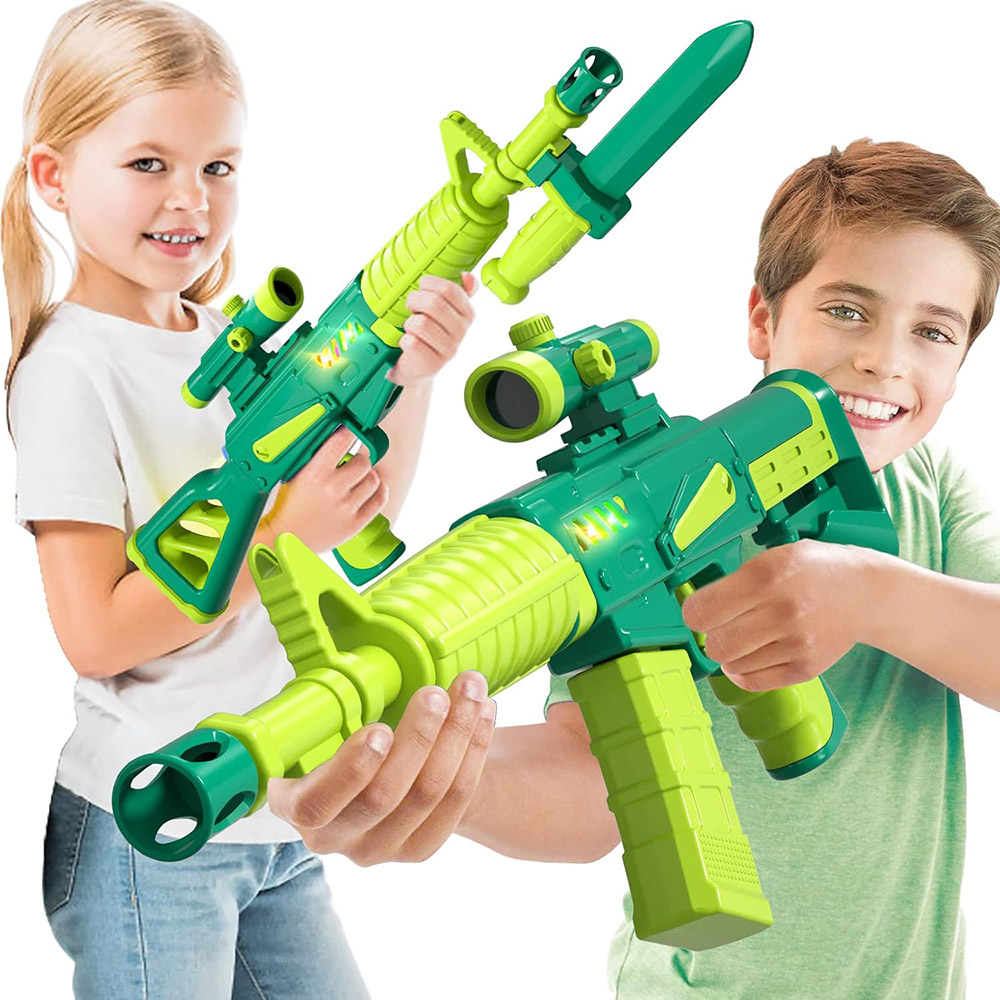
\includegraphics[width=\textwidth]{images/Giocattolo.jpg}
      \caption{Replica giocattolo in plastica}
      \label{fig:giocattolo}
  \end{subfigure}
  \hfill
  \begin{subfigure}[t]{0.31\textwidth}
      \centering
      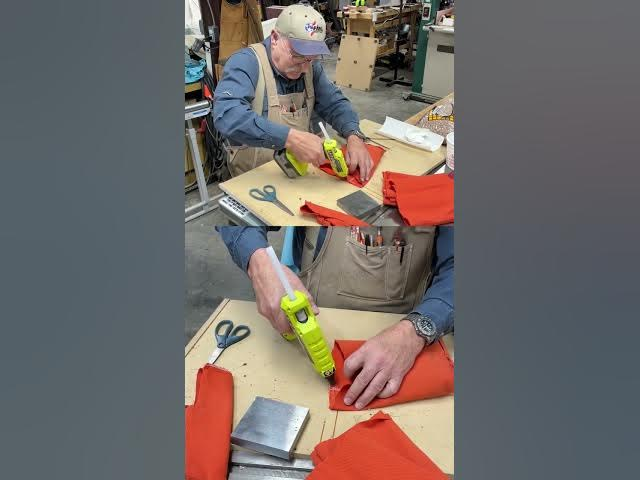
\includegraphics[width=\textwidth]{images/Ambigua.jpg}
      \caption{Caso ambiguo (escluso)}
      \label{fig:ambigua}
  \end{subfigure}

  \caption{Esempi tipici di classificazione: (a) arma reale, (b) replica giocattolo, (c) immagine ambigua esclusa con criterio conservativo.}
  \label{fig:weapon-toy-examples}
\end{figure}


\bigskip

La procedura descritta ha generato un file CSV contenente per ciascuna immagine un’etichetta binaria nella colonna \texttt{manual\_is\_real\_weapon}, che costituisce il riferimento oggettivo per la valutazione delle performance dei modelli AI nei test di robustezza e generalizzazione Out-of-Distribution.





\subsection{Out-of-Distribution Detection come test preliminare}
\label{sec:ood-pre-test}

Per garantire la validità dei test condotti sugli strumenti AI-based in ambito forense, è stato introdotto un passaggio preliminare di \textbf{Out-of-Distribution (OOD) Detection}. L'obiettivo è identificare immagini potenzialmente fuori distribuzione, ovvero contenuti visivi che differiscono in modo sostanziale dal dominio previsto (es. armi da fuoco reali) e che potrebbero compromettere l'affidabilità dei modelli.

Tale fase costituisce un filtro semantico a monte dell'inferenza AI, migliorando la robustezza del processo complessivo. La rilevazione è stata effettuata tramite modelli vision-language in modalità \textit{zero-shot} (CLIP, BLIP), con successiva validazione manuale da parte dell'autore. I dettagli tecnici e il codice utilizzato per l'annotazione manuale sono riportati in Appendice~\ref{appendix:clip-ood-script}.






\subsection{Valutazione comparativa tra classificazione automatica e annotazione manuale}
\label{sec:valutazione-ood}

Per valutare la bontà del filtraggio automatico delle immagini Out-of-Distribution (OOD), è stata condotta una comparazione tra i risultati del modello \textbf{CLIP ViT-B/32} in modalità \textit{zero-shot} e un'annotazione \textbf{manuale interattiva}, effettuata dall'autore mediante interfaccia grafica batch.

L'analisi ha coinvolto un totale di \textbf{1000 immagini} provenienti da cinque dataset eterogenei. Ogni immagine è stata classificata automaticamente come \texttt{in-distribution} o \texttt{OOD} tramite confronto con prompt semantici (arma, oggetto, persona, ecc.), quindi sottoposta ad etichettatura binaria manuale: \texttt{arma reale} oppure \texttt{non arma}.

\medskip

I risultati aggregati per il modello CLIP sono riportati nella Tabella~\ref{tab:ood-clip}:

\begin{table}[H]
\centering
\begin{tabular}{l r}
\toprule
\textbf{Metrica} & \textbf{Valore} \\
\midrule
Totale immagini analizzate & 1000 \\
Immagini OOD secondo CLIP & 246 \\
Immagini OOD secondo annotazione manuale & 127 \\
Immagini classificate in-distribution da CLIP & 754 \\
Veri positivi (OOD corrette) & 109 \\
Falsi positivi (CLIP = OOD, ma in realtà arma) & 137 \\
Falsi negativi (CLIP = ID, ma in realtà non arma) & 18 \\
\midrule
\textbf{Precisione} & 44.3\% \\
\textbf{Richiamo (Recall)} & 85.8\% \\
\textbf{F1-Score} & 58.4\% \\
\bottomrule
\end{tabular}
\caption{Confronto tra classificazione automatica (CLIP) e annotazione manuale per la rilevazione di immagini fuori distribuzione.}
\label{tab:ood-clip}
\end{table}

Come evidenziato, l’approccio CLIP mostra un’elevata \textbf{capacità di richiamo} (\texttt{Recall = 85.8\%}), indicando una forte propensione del modello ad includere tutte le immagini effettivamente OOD. Tuttavia, la \textbf{bassa precisione} (\texttt{Precision = 44.3\%}) segnala una tendenza alla sovra-classificazione: numerose immagini effettivamente pertinenti (armi reali) vengono erroneamente considerate fuori distribuzione.

\medskip

\noindent Questo comportamento suggerisce una \textbf{scarsa specificità semantica} del modello rispetto a contesti visivi ambigui o sfumati, un limite noto per i modelli \textit{zero-shot} non adattati al dominio. Il valore intermedio del \texttt{F1-Score = 58.4\%} riflette un compromesso sbilanciato tra sensibilità e precisione, evidenziando l’opportunità di raffinare i prompt o integrare fasi di fine-tuning.








\subsection{Rilevamento OOD mediante BLIP}
\label{sec:ood-blip}

Il modello \textbf{BLIP -Bootstrapping Language-Image Pretraining } è un framework multimodale avanzato, progettato per apprendere rappresentazioni visuo-linguistiche in maniera efficiente mediante \textit{image-text matching} e \textit{captioning}. In questo studio, BLIP è stato impiegato in modalità \textit{zero-shot}, utilizzando prompt descrittivi per discriminare le immagini appartenenti o meno al dominio delle armi.

L’analisi sulle stesse \textbf{1000 immagini} ha mostrato un totale di \textbf{358 immagini classificate come OOD} da BLIP, contro le 127 indicate dall’annotazione manuale. L’accuratezza complessiva del modello BLIP nella classificazione OOD/in-distribution è risultata pari al \textbf{74.5\%}.

\medskip

Sebbene meno aggressivo rispetto a CLIP nella rilevazione OOD, BLIP ha comunque prodotto un numero elevato di falsi positivi. Questo comportamento potrebbe essere attribuito a una maggiore sensibilità del modello verso il contesto visivo e linguistico, ma anche a una certa difficoltà nel distinguere contenuti semantici specifici in domini visivamente simili.




\subsection{Rilevamento OOD mediante EfficientNet}
\label{sec:ood-efficientnet}

Il modello \textbf{EfficientNet} è una rete convoluzionale ottimizzata per efficienza e accuratezza, basata su uno scaling uniforme di profondità, larghezza e risoluzione~\cite{tan2019efficientnet}. In questa sperimentazione, EfficientNet è stato adattato al compito OOD tramite una procedura di classificazione binaria: la predizione di classe è stata confrontata con un dizionario predefinito di categorie target per rilevare immagini incongruenti.

EfficientNet ha identificato \textbf{314 immagini come OOD}, ottenendo una \textbf{accuracy complessiva del 57.3\%} rispetto alle etichette manuali. Si osserva una maggiore propensione a classificare immagini ambigue come in-distribution, con un conseguente incremento dei falsi negativi.

\medskip

Questo risultato evidenzia i limiti dei modelli CNN tradizionali nell’affrontare il problema OOD in contesti generalizzati, soprattutto in assenza di meccanismi di inferenza semantica esplicita come nei modelli vision-language.




\subsection{Rilevamento OOD mediante ResNet+SVM}
\label{sec:ood-resnet-svm}

L’approccio \textbf{ResNet+SVM} si basa sull’estrazione di feature visuali tramite una \textit{ResNet-18} pre-addestrata, seguita dalla classificazione binaria tramite un \textit{Support Vector Machine} (SVM). Le feature sono state ridotte dimensionalmente e normalizzate prima della classificazione, con la decisione OOD derivata dalla distanza della predizione rispetto alle classi note.

Questo sistema ha mostrato un comportamento diametralmente opposto rispetto a CLIP e BLIP: ben \textbf{861 immagini} su 1000 sono state etichettate come \texttt{OOD}, con un’\textbf{accuracy complessiva pari al 25.2\%}. Il modello ha quindi sovrastimato in maniera drastica la presenza di immagini fuori distribuzione, fallendo nella generalizzazione.

\medskip

Questa limitata capacità discriminativa è verosimilmente legata alla mancanza di un'adeguata rappresentazione semantica nei descrittori visivi estratti, nonché alla rigidità del classificatore SVM nel contesto OOD. Il risultato suggerisce che pipeline basate su SVM classici siano poco adatte per compiti di open-world classification senza specifico addestramento.



\section{Valutazione comparativa globale dei classificatori}
\label{sec:global-evaluation}

Per valutare in modo sistematico le capacità discriminative dei modelli AI utilizzati per il rilevamento di immagini \textit{out-of-distribution} (OOD), è stata condotta un’analisi comparativa basata su un test set di 1000 immagini, annotate manualmente come \texttt{arma reale} o \texttt{non arma}. I risultati ottenuti dai classificatori automatici sono stati confrontati con tale etichettatura, considerata come \textit{ground truth}.

\subsection{Metriche e approccio comparativo}

Ogni modello ha prodotto una classificazione binaria (\texttt{OOD} o \texttt{in-distribution}), confrontata con l’etichetta \texttt{manual\_is\_real\_weapon}. In questo contesto, un’immagine è considerata OOD se non rappresenta un’arma reale. Le metriche calcolate per ciascun classificatore includono:

\begin{itemize}
  \item \textbf{Accuracy} — percentuale di immagini correttamente classificate rispetto all’annotazione manuale;
  \item \textbf{Precision} — proporzione di immagini etichettate come OOD che sono effettivamente non armi;
  \item \textbf{Recall} — capacità del modello di individuare tutte le immagini effettivamente OOD;
  \item \textbf{F1-Score} — media armonica tra precision e recall.
\end{itemize}

\subsection{Risultati aggregati}

La Tabella~\ref{tab:ood-global-comparison} sintetizza i risultati ottenuti.

\begin{table}[H]
\centering
\begin{tabular}{lcccc}
\toprule
\textbf{Strumento} & \textbf{Accuracy (\%)} & \textbf{Precision (\%)} & \textbf{Recall (\%)} & \textbf{F1-Score (\%)} \\
\midrule
CLIP           & 86.50 & 48.37 & 93.70 & 63.81 \\
BLIP           & 74.50 & 32.12 & 90.55 & 47.42 \\
EfficientNet   & 57.30 &  2.23 &  5.51 &  3.17 \\
ResNet+SVM     & 25.20 & 13.94 & 94.49 & 24.29 \\
\bottomrule
\end{tabular}
\caption{Confronto tra classificatori automatici e annotazione manuale nel rilevamento di immagini OOD.}
\label{tab:ood-global-comparison}
\end{table}

Come mostrato nella Tabella~\ref{tab:ood-global-comparison}, il modello \textbf{CLIP ViT-B/32} si conferma il più bilanciato, con un’accuratezza complessiva del 86.5\% e un buon compromesso tra richiamo (93.7\%) e precisione (48.4\%), rendendolo adatto a contesti in cui la minimizzazione dei falsi negativi è prioritaria.

Il modello \textbf{BLIP} mostra prestazioni inferiori su tutte le metriche, suggerendo una maggiore fragilità nel riconoscimento semantico. Al contrario, \textbf{EfficientNet} e \textbf{ResNet+SVM} evidenziano un comportamento fortemente sbilanciato: in particolare, ResNet+SVM ottiene un elevato valore di recall (94.5\%) ma a discapito della precisione (13.9\%), indicando una marcata tendenza alla sovra-classificazione.

Questi risultati confermano che i modelli \textit{vision-language} come CLIP e BLIP sono attualmente più efficaci nel rilevamento di contenuti fuori distribuzione, specialmente in configurazioni zero-shot, mentre i modelli CNN tradizionali risultano meno adatti a questo compito senza un fine-tuning specifico.

\subsection{Analisi qualitativa dei risultati}

Il modello CLIP si distingue per l’elevata sensibilità, individuando quasi tutte le immagini realmente OOD, ma a costo di una precisione ridotta: molte immagini raffiguranti armi vengono erroneamente classificate come fuori distribuzione. Tale comportamento lo rende adatto come filtro ad alta copertura, da affiancare a un secondo livello di verifica.

EfficientNet e ResNet+SVM evidenziano una scarsa generalizzazione, con accuratezze complessive basse e prestazioni instabili. BLIP si colloca in una posizione intermedia: pur non essendo stato progettato per classificazione binaria, ha mostrato buone capacità di matching semantico nel confronto visivo.





\subsection{Conclusioni comparative}

L’analisi evidenzia l’importanza di una \textbf{combinazione tra classificazione automatica e revisione manuale}, soprattutto in ambito forense, dove la mancata identificazione di un’evidenza (falso negativo) può compromettere l’intero processo investigativo. In questo scenario, strumenti come CLIP possono essere adottati come \textit{moduli di pre-screening} sensibili, integrabili in pipeline più ampie che prevedano successivi passaggi di validazione umana o algoritmica.









